\documentclass[a4paper, 12pt]{article}
\usepackage[utf8]{inputenc}
\usepackage[russian]{babel}
\usepackage{vmargin}
\usepackage{amsmath}
\usepackage{amssymb}
\usepackage{latexsym}
\usepackage{natbib}
\usepackage{graphicx}
\usepackage{booktabs}
\setpapersize{A4}
\setmarginsrb{2cm}{1.5cm}{1cm}{1.5cm}{0pt}{0mm}{0pt}{13mm}
\usepackage{indentfirst}
\DeclareGraphicsExtensions{.pdf,.png,.jpg}
\graphicspath{{pictures/}}
\binoppenalty=1000
\relpenalty=1000
\usepackage[unicode, pdftex,pdfborder=0 0 0,colorlinks, linkcolor=black]{hyperref}
\usepackage[utf8]{inputenc}
\usepackage[english,russian]{babel}

\usepackage{graphicx}
\usepackage{hyperref}
\usepackage{amsmath}
\sloppy

\begin{document}


\title{Численное решение одномерного уравнения Навье-Стокса с использованием схемы с центральными разностями (последовательная) (\(\rho\), \(\rho\)u)}

\maketitle
\section{Постановка задачи}
\begin{equation*}
 \begin{cases}
\frac{\partial \rho}{\partial t}+  \frac{\partial \rho u}{\partial x}=0
\\
\rho \frac{\partial u}{\partial t}+\rho u \frac{\partial u}{\partial x}+ \frac{\partial p}{\partial x}=\mu \frac{\partial^{2}u}{\partial x^{2}} +\rho f
\\
p=p(\rho)
 \end{cases}
\end{equation*}

\(\mu\) - известный коэффифциент вязкости газа

\(\rho\), \(u\) - функционалы плотности и скорости(газа): (\(t\), \(x\)) \(\in\) [0, \(T\)] \(*\) [0, \(X\)]

\(p\) = \(C\)\(\rho\) - давление газа

\(f\) - вектор внешних сил

\bigskip
\section{Описание схемы}
Для поиска численного решения задачи можно использовать разностную схему, в которой при апроксимации членов используются центральные разности, а функции H, V на последующем слое ищутся путем
решения двух систем линейных уравнений методом прогонки.

\begin{equation*}
\begin{cases}
H_{t,0}+0.5((V\stackrel{\wedge}{H})_{x,0}+H_{0}V{x,0})-0.5h((HV)_{x,\overline{x},1}-0.5(HV)_{x,\overline{x},2}+H_{0}(V_{x, \overline{x},1}-0.5V_{x, \overline{x},2}))=0
\\
H_{t}+ 0.5(V \stackrel{\wedge}{H}_{\stackrel{0}{x}}+(V \stackrel{\wedge}{H})_{\stackrel{0}{x}}+HV{\stackrel{0}{x}})=0,x \in \omega_{h}
\\
H_{t,M}+0.5((V\stackrel{\wedge}{H})_{\overline x,M}+H_{M}V{\overline x,M})-0.5h((HV)_{x,\overline{x},M-1}-0.5(HV)_{x,\overline{x},M-2}+
\\
+H_{M}(V_{x, \overline{x},M-1}-0.5V_{x, \overline{x},M-2}))=0
\\
(HV)_{t}+\frac{2}{3}( \stackrel{\wedge}{H} V \stackrel{\wedge}{V})_{\stackrel{0}{x}} 
+ \frac{2}{3} \stackrel{\wedge}{H} V \stackrel{\wedge}{V}_{\stackrel{0}{x}}
+ \frac{{V}^{2}}{3}\stackrel{\wedge}{H}_{\stackrel{0}{x}}
+ p( \stackrel{\wedge}{H})_{\stackrel{0}{x}} = 
\mu \stackrel{\wedge}{V}_{x \overline x}
+\stackrel{\wedge}{H}f ,   x \in \omega_{h}
\end{cases}
\end{equation*}

\(\omega_{h}\) - внутренние узлы сетки 
В качестве значений решения уравнений на нулевом слое берутся функции \(\rho_{0}\) и \(u_{0}\):

    $$ H^{0}_{m} = (\rho_{0})_{m},  V^{0}_{m} = (u_{0})_{m},        m=0,1,\dots,M$$

Граничные условия скорости равны нулю:
$$ V^{n}_{0} =  V^{n}_{M} = 0,    m=1,\dots,N $$

\section{Координатная запись уравнений}
\begin{equation*}
\begin{cases}
\frac{H_{0}^{n+1}-H_{0}^{n}}{t}+\frac{1}{2}(\frac{V_{1}^{n}H_{1}^{n+1}-V_{0}^{n}H_{0}^{n+1}}{h}+H_{0}^{n}\frac{V_{1}^{n}-V_{0}^{n}}{h})-
\\
-\frac{h}{2} (\frac{H_{2}^{n}V_{2}^{n}-2H_{1}^{n}V_{1}^{n}+H_{0}^{n}V_{0}^{n}}{h^{2}}-\frac{1}{2}\frac{H_{3}^{n}V_{3}^{n}-2H_{2}^{n}V_{2}^{n}+H_{1}^{n}V_{1}^{n}}{h^{2}}+H_{0}^{n}(\frac{V_{2}^{n}-2V_{1}^{n}+V_{0}^{n}}{h^2}-\frac{V_{3}^{n}-2V_{2}^{n}+V_{1}^{n}}{2h^{2}}))=0
\\
\\
\frac{H_{m}^{n+1}-H_{}m^{n}}{t}+\frac{1}{2}(V_{m}^{n}\frac{H_{m+1}^{n+1}-H_{m-1}^{n+1}}{2h}+\frac{V_{m+1}^{n}H_{m+1}^{n+1}-V_{m-1}^{n}H_{m-1}^{n+1}}{2h}+H_{m}^{n}\frac{V_{m+1}^{n}-V_{m-1}^{n}}{2h})=0
\\
\\
 \frac{H_{M}^{n+1}-H_{M}^{n}}{t}+\frac{1}{2}(\frac{V_{M}^{n}H_{M}^{n+1}-V_{M-1}^{n}H_{M-1}^{n+1}}{h}+H_{M}^{n}\frac{V_{M}^{n}-V_{M-1}^{n}}{h})-
-\frac{h}{2} (\frac{H_{M}^{n}V_{M}^{n}-2H_{M-1}^{n}V_{M-1}^{n}+H_{M-2}^{n}V_{M-2}^{n}}{h^{2}}- \\-\frac{1}{2}\frac{H_{M-1}^{n}V_{M-1}^{n}-2H_{M-2}^{n}V_{M-2}^{n}+H_{M-3}^{n}V_{M-3}^{n}}{h^{2}}+H_{M}^{n}(\frac{V_{M}^{n}-2V_{M-1}^{n}+V_{M-2}^{n}}{h^2}-\frac{V_{M-1}^{n}-2V_{M-2}^{n}+V_{M-3}^{n}}{2h^{2}}))=0
\\
\\
\frac{H_{m}^{n+1}V_{m}^{n+1}-H_{m}^{n}V_{m}^{n}}{t}
+\frac{2}{3}(\frac{H_{m+1}^{n+1} V_{m+1}^{n} V_{m+1}^{n+1} 
                    - H_{m-1}^{n+1} V_{m-1}^{n} V_{m-1}^{n+1}} 
                  {2h})
+\frac{2}{3}H_{m}^{n+1} V_{m}^{n} (\frac{V_{m+1}^{n+1} - V_{m-1}^{n+1}} 
                                         {2h})
+ (\frac{{V_{m}^{n}}^{2}}{3} + p)  (\frac{H_{m+1}^{n+1} - H_{m-1}^{n+1}} 
                                         {2h}))
                  
=
\\=\mu\frac{V_{m+1}^{n+1} - 2 V_{m}^{n+1} + V_{m}^{n+1}}{h^{2}} + H_{m}^{n+1}f
\end{cases}
\end{equation*}

Выделяя коэффициенты при членах \(H^{n+1}_{m-1}\), \(H^{n+1}_{m}\), \(H^{n+1}_{m+1}\) из первых трёх уравнений системы, получим трёхдиагональную матрицу(первые два уравнения как раз сделают нашу матрицу трёхдиагональной, т.к. там участвует всего два члена). Аналогично выделяя из 4-го уравнения \(V^{n+1}_{m-1}\), \(V^{n+1}_{m}\), \(V^{n+1}_{m+1}\) получим трёхдиагональную матрицу(ещё два уравнения берутся из \(V^{n}_{0} = 0\) и \(V^{n}_{M} = 0\))

\section{Расчёт гладкого решения}

Для того чтобы расчитать гладкое решение зададим функции:
$$
\widetilde{\rho}=e^{t}(cos(\frac{\pi x}{10})+1.5),
\text{ }
\widetilde {u}=cos(2\pi t)sin(\pi \frac{x^{2}}{100})
$$
Определим функции $f_{0}$ и $f$ так, чтобы они удовлетворяли системе:
\begin{equation*}
 \begin{cases}
\frac{\partial \widetilde{\rho}}{\partial t}+  \frac{\partial \widetilde{\rho} \widetilde{u}}{\partial x}=f_{0}
\\
\widetilde{\rho} \frac{\partial \widetilde{u}}{\partial t}+\widetilde{\rho} \widetilde{u} \frac{\partial \widetilde{u}}{\partial x}+ \frac{\partial \widetilde{p}}{\partial x}=\mu \frac{\partial^{2}\widetilde{u}}{\partial x^{2}} +\widetilde{\rho} f
\\
p=p(\widetilde{\rho})
 \end{cases}
\end{equation*}
Проведя подстановку и соответствующие вычисления найдем эти функции:
\begin{equation*}
 \begin{cases}
f_{0}(t,x)=e^{t}(cos( \frac{\pi x}{10})+1.5)+e^{t}cos(2\pi t)( -\frac{\pi}{10}sin(\frac{\pi x}{10})sin( \frac{\pi x^{2}}{100})+ \frac{\pi x}{50}cos(\frac{\pi x^{2}}{100})(cos( \frac{\pi x}{10})+1.5)
\\ \\

f(t,x)=(-e^{t}(cos( \frac{\pi x}{10})+1.5)2 \pi sin(2 \pi t)sin( \frac{\pi x^{2}}{100})+\frac{\pi t}{50}e^{t}(cos( \frac{\pi x}{10})+1.5) (cos(2 \pi t))^{2} sin( \frac{\pi x^{2}}{100})cos(\frac{\pi x^{2}}{100})- \\
-p(\frac{\pi}{10})e^{t}sin( \frac{\pi x}{10})-\frac{\mu \pi}{50} cos(2\pi t)(cos(\frac{\pi x^{2}}{100})-\frac{x^{2} \pi}{50}sin((\frac{\pi x^{2}}{100}))))/(e^{t}(cos(\frac{\pi x}{10})+1.5))
 \end{cases}
\end{equation*}

Таким образом,  имеется дифференциальная задача для системы с начальными и граничными условиями:
\begin{equation*}
 \begin{cases}
\widetilde{\rho}(0,x)=cos(\frac{\pi x}{10})+1.5, x \in [0,10]
\\
\widetilde {u}(0,x)=sin(\pi \frac{x^{2}}{100}), x \in [0,10]
\\
\widetilde {u}(t,0)=\widetilde {u}(t,10)=0, t \in [0,1]
 \end{cases}
\end{equation*}
\\ 
\\
Запустим программу и составим таблицы ошибок численного решения с теоретическим для плотности и скорости в нормах $||\text{ }||_{C_{h}},\text{ }||\text{ }||_{L_{2}},\text{ }||\text{ }||_{W}$ при  различных значениях   С$=1,10,100$ и $\mu=0.1,0.01,0.001$.
\\
\subsection{Таблицы ошибок}
Mu=0.1  C=1 Норма=L2 H(Плотность):


\begin{tabular}{lllll}
\toprule
{} &         10    &         100   &         1000  &         10000 \\
\midrule
10    &  4.696012e-01 &  4.676729e-01 &  4.676547e-01 &  4.676542e-01 \\
100   &  5.273774e-02 &  4.794685e-02 &  4.793345e-02 &  4.793332e-02 \\
1000  &  2.061029e-02 &  4.822147e-03 &  4.807590e-03 &  4.807479e-03 \\
10000 &  1.983687e-02 &  5.248298e-04 &  4.810054e-04 &  4.808928e-04 \\
\bottomrule
\end{tabular}



\bigskip
\bigskip
\bigskip


Mu=0.1  C=1 Норма=L2 V(Скорость):


\begin{tabular}{lllll}
\toprule
{} &         10    &         100   &         1000  &         10000 \\
\midrule
10    &  4.875196e-02 &  2.988319e-02 &  2.970035e-02 &  2.969852e-02 \\
100   &  2.258236e-02 &  8.504889e-04 &  7.253258e-04 &  7.243288e-04 \\
1000  &  2.216811e-02 &  2.495879e-04 &  6.949198e-05 &  6.912976e-05 \\
10000 &  2.214678e-02 &  2.309446e-04 &  7.547881e-06 &  6.940393e-06 \\
\bottomrule
\end{tabular}



\bigskip
\bigskip
\bigskip


Mu=0.01  C=1 Норма=L2 H(Плотность):


\begin{tabular}{lllll}
\toprule
{} &         10    &         100   &         1000  &         10000 \\
\midrule
10    &  4.693622e-01 &  4.680585e-01 &  6.490445e-01 &  5.836857e-01 \\
100   &  5.309688e-02 &  4.801370e-02 &  4.800133e-02 &  4.800121e-02 \\
1000  &  2.166696e-02 &  4.828824e-03 &  4.814649e-03 &  4.814546e-03 \\
10000 &  2.094877e-02 &  5.282214e-04 &  4.817075e-04 &  4.816021e-04 \\
\bottomrule
\end{tabular}



\bigskip
\bigskip
\bigskip


Mu=0.01  C=1 Норма=L2 V(Скорость):


\begin{tabular}{lllll}
\toprule
{} &         10    &         100   &         1000  &         10000 \\
\midrule
10    &  5.029442e-02 &  3.087900e-02 &  1.917698e+00 &  4.204071e-02 \\
100   &  2.354953e-02 &  1.037940e-03 &  9.277028e-04 &  9.268492e-04 \\
1000  &  2.311536e-02 &  2.684276e-04 &  9.006968e-05 &  8.974294e-05 \\
10000 &  2.309261e-02 &  2.431423e-04 &  9.537925e-06 &  8.992415e-06 \\
\bottomrule
\end{tabular}



\bigskip
\bigskip
\bigskip


Mu=0.001  C=1 Норма=L2 H(Плотность):


\begin{tabular}{lllll}
\toprule
{} &         10    &         100   &         1000  &         10000 \\
\midrule
10    &  4.693392e-01 &  4.681079e-01 &  2.101289e+05 &  6.689137e+00 \\
100   &  5.313843e-02 &  4.802108e-02 &  4.800866e-02 &  2.831079e+51 \\
1000  &  2.178340e-02 &  4.829571e-03 &  4.815410e-03 &  4.815307e-03 \\
10000 &  2.107080e-02 &  5.287424e-04 &  4.817831e-04 &  4.816785e-04 \\
\bottomrule
\end{tabular}



\bigskip
\bigskip
\bigskip


Mu=0.001  C=1 Норма=L2 V(Скорость):


\begin{tabular}{lllll}
\toprule
{} &         10    &         100   &         1000  &         10000 \\
\midrule
10    &  5.046303e-02 &  3.099334e-02 &  1.048840e+01 &  1.108761e+00 \\
100   &  2.365315e-02 &  1.058706e-03 &  9.495971e-04 &  2.373660e+01 \\
1000  &  2.321639e-02 &  2.706002e-04 &  9.228166e-05 &  9.195584e-05 \\
10000 &  2.319345e-02 &  2.445016e-04 &  9.755249e-06 &  9.212892e-06 \\
\bottomrule
\end{tabular}



\bigskip
\bigskip
\bigskip


Mu=0.1  C=10 Норма=L2 H(Плотность):


\begin{tabular}{lllll}
\toprule
{} &         10    &         100   &         1000  &         10000 \\
\midrule
10    &  5.012199e-01 &  9.026897e-01 &  1.332887e+00 &  5.881042e-01 \\
100   &  7.313454e-02 &  5.014497e-02 &  4.997401e-02 &  4.997231e-02 \\
1000  &  3.731945e-02 &  5.190596e-03 &  5.009589e-03 &  5.007854e-03 \\
10000 &  3.481758e-02 &  7.325545e-04 &  5.026531e-04 &  5.009082e-04 \\
\bottomrule
\end{tabular}



\bigskip
\bigskip
\bigskip


Mu=0.1  C=10 Норма=L2 V(Скорость):


\begin{tabular}{lllll}
\toprule
{} &         10    &         100   &         1000  &         10000 \\
\midrule
10    &  1.569949e-01 &  2.877876e+00 &  4.068294e-01 &  6.828291e-01 \\
100   &  8.370070e-02 &  7.345906e-03 &  6.609983e-03 &  6.602657e-03 \\
1000  &  7.800496e-02 &  1.406512e-03 &  6.541825e-04 &  6.468310e-04 \\
10000 &  7.744941e-02 &  8.367915e-04 &  7.200164e-05 &  6.461758e-05 \\
\bottomrule
\end{tabular}



\bigskip
\bigskip
\bigskip


Mu=0.01  C=10 Норма=L2 H(Плотность):


\begin{tabular}{lllll}
\toprule
{} &         10    &         100   &         1000  &         10000 \\
\midrule
10    &  5.022084e-01 &  1.423619e+05 &  8.159490e+02 &  1.626592e+01 \\
100   &  7.327862e-02 &  5.023381e-02 &  8.824849e+18 &  2.323187e+57 \\
1000  &  3.737192e-02 &  5.199727e-03 &  5.018538e-03 &  5.016802e-03 \\
10000 &  3.486279e-02 &  7.338343e-04 &  5.035502e-04 &  5.018037e-04 \\
\bottomrule
\end{tabular}



\bigskip
\bigskip
\bigskip


Mu=0.01  C=10 Норма=L2 V(Скорость):


\begin{tabular}{lllll}
\toprule
{} &         10    &         100   &         1000  &         10000 \\
\midrule
10    &  1.565878e-01 &  5.941192e+01 &  1.291210e+02 &  3.461202e+00 \\
100   &  8.395313e-02 &  7.292156e-03 &  1.032459e+02 &  1.677696e+03 \\
1000  &  7.826410e-02 &  1.405301e-03 &  6.488478e-04 &  6.414393e-04 \\
10000 &  7.770867e-02 &  8.391346e-04 &  7.152280e-05 &  6.408480e-05 \\
\bottomrule
\end{tabular}



\bigskip
\bigskip
\bigskip


Mu=0.001  C=10 Норма=L2 H(Плотность):


\begin{tabular}{lllll}
\toprule
{} &         10    &         100   &         1000  &         10000 \\
\midrule
10    &  5.023105e-01 &  1.880213e+03 &  3.851973e+07 &  2.061678e+08 \\
100   &  7.329301e-02 &  5.024290e-02 &  7.588565e+30 &  1.569206e+69 \\
1000  &  3.737683e-02 &  5.200660e-03 &  5.019454e-03 &          -nan \\
10000 &  3.486694e-02 &  7.339606e-04 &  5.036420e-04 &  5.018953e-04 \\
\bottomrule
\end{tabular}



\bigskip
\bigskip
\bigskip


Mu=0.001  C=10 Норма=L2 V(Скорость):


\begin{tabular}{lllll}
\toprule
{} &         10    &         100   &         1000  &         10000 \\
\midrule
10    &  1.565492e-01 &  6.564508e+01 &  3.606669e+02 &  5.992662e+02 \\
100   &  8.397854e-02 &  7.287299e-03 &  3.929503e+02 &  9.418635e+02 \\
1000  &  7.828992e-02 &  1.405225e-03 &  6.483702e-04 &          -nan \\
10000 &  7.773447e-02 &  8.393762e-04 &  7.148029e-05 &  6.403716e-05 \\
\bottomrule
\end{tabular}



\bigskip
\bigskip
\bigskip


Mu=0.1  C=100 Норма=L2 H(Плотность):


\begin{tabular}{lllll}
\toprule
{} &         10    &         100   &         1000  &         10000 \\
\midrule
10    &  6.892732e-01 &  1.695477e+05 &  2.067894e+02 &  6.274060e+01 \\
100   &  1.848169e-01 &  5.844659e-02 &  6.097917e+56 &  1.569375e+62 \\
1000  &  1.436575e-01 &  6.776485e-03 &  5.750473e-03 &  5.740913e-03 \\
10000 &  1.399390e-01 &  1.822592e-03 &  5.837462e-04 &  5.741137e-04 \\
\bottomrule
\end{tabular}



\bigskip
\bigskip
\bigskip


Mu=0.1  C=100 Норма=L2 V(Скорость):


\begin{tabular}{lllll}
\toprule
{} &         10    &         100   &         1000  &         10000 \\
\midrule
10    &  5.988637e-01 &  6.676197e+02 &  5.718412e+01 &  6.314213e+02 \\
100   &  6.792977e-02 &  5.473185e-02 &  1.279158e+03 &  5.070745e+03 \\
1000  &  9.111640e-02 &  4.898343e-03 &  5.415732e-03 &  5.421298e-03 \\
10000 &  9.448411e-02 &  6.370485e-04 &  5.354648e-04 &  5.409874e-04 \\
\bottomrule
\end{tabular}



\bigskip
\bigskip
\bigskip


Mu=0.01  C=100 Норма=L2 H(Плотность):


\begin{tabular}{lllll}
\toprule
{} &         10    &         100   &         1000  &          10000 \\
\midrule
10    &  6.903202e-01 &  1.946647e+08 &  1.744581e+08 &   1.342455e+09 \\
100   &  1.850824e-01 &  5.850591e-02 &  9.040434e+73 &  1.619640e+104 \\
1000  &  1.438637e-01 &  6.784032e-03 &  5.755983e-03 &           -nan \\
10000 &  1.401390e-01 &  1.825028e-03 &  5.843136e-04 &   5.746605e-04 \\
\bottomrule
\end{tabular}



\bigskip
\bigskip
\bigskip


Mu=0.01  C=100 Норма=L2 V(Скорость):


\begin{tabular}{lllll}
\toprule
{} &         10    &         100   &         1000  &         10000 \\
\midrule
10    &  6.024827e-01 &  1.099879e+03 &  6.972934e+02 &  6.449024e+03 \\
100   &  6.784567e-02 &  5.506345e-02 &  5.898998e+02 &  3.429337e+03 \\
1000  &  9.124946e-02 &  4.929974e-03 &  5.448898e-03 &          -nan \\
10000 &  9.465230e-02 &  6.357584e-04 &  5.387688e-04 &  5.443044e-04 \\
\bottomrule
\end{tabular}



\bigskip
\bigskip
\bigskip


Mu=0.001  C=100 Норма=L2 H(Плотность):


\begin{tabular}{lllll}
\toprule
{} &         10    &         100   &         1000  &         10000 \\
\midrule
10    &  6.904225e-01 &  1.822857e+09 &  3.449237e+09 &  7.086286e+02 \\
100   &  1.851091e-01 &  5.851193e-02 &  6.652407e+78 &  2.399980e+98 \\
1000  &  1.438845e-01 &  6.784796e-03 &  5.756542e-03 &          -nan \\
10000 &  1.401592e-01 &  1.825274e-03 &  5.843711e-04 &  5.747160e-04 \\
\bottomrule
\end{tabular}



\bigskip
\bigskip
\bigskip


Mu=0.001  C=100 Норма=L2 V(Скорость):


\begin{tabular}{lllll}
\toprule
{} &         10    &         100   &         1000  &         10000 \\
\midrule
10    &  6.028481e-01 &  4.193698e+02 &  2.259071e+02 &  1.238218e+02 \\
100   &  6.783802e-02 &  5.509685e-02 &  6.411388e+02 &  3.794281e+03 \\
1000  &  9.126407e-02 &  4.933165e-03 &  5.452239e-03 &          -nan \\
10000 &  9.467046e-02 &  6.356328e-04 &  5.391017e-04 &  5.446386e-04 \\
\bottomrule
\end{tabular}



\bigskip
\bigskip
\bigskip


Mu=0.1  C=1 Норма=W H(Плотность):


\begin{tabular}{lllll}
\toprule
{} &         10    &         100   &         1000  &         10000 \\
\midrule
10    &  2.266352e-01 &  2.242783e-01 &  2.243384e-01 &  2.243389e-01 \\
100   &  3.339934e-03 &  2.369863e-03 &  2.369207e-03 &  2.369199e-03 \\
1000  &  9.218857e-04 &  2.401876e-05 &  2.385377e-05 &  2.385293e-05 \\
10000 &  8.910033e-04 &  3.310484e-07 &  2.387876e-07 &  2.386945e-07 \\
\bottomrule
\end{tabular}



\bigskip
\bigskip
\bigskip


Mu=0.1  C=1 Норма=W V(Скорость):


\begin{tabular}{lllll}
\toprule
{} &         10    &         100   &         1000  &         10000 \\
\midrule
10    &  4.636821e-03 &  1.678804e-03 &  1.656712e-03 &  1.656500e-03 \\
100   &  1.101281e-03 &  1.163023e-06 &  7.858796e-07 &  7.833380e-07 \\
1000  &  1.067990e-03 &  1.396659e-07 &  6.967660e-09 &  6.916825e-09 \\
10000 &  1.066495e-03 &  1.291266e-07 &  8.436066e-11 &  6.980559e-11 \\
\bottomrule
\end{tabular}



\bigskip
\bigskip
\bigskip


Mu=0.01  C=1 Норма=W H(Плотность):


\begin{tabular}{lllll}
\toprule
{} &         10    &         100   &         1000  &         10000 \\
\midrule
10    &  2.266125e-01 &  2.246461e-01 &  1.344835e+03 &  2.011295e+04 \\
100   &  3.444780e-03 &  2.377525e-03 &  2.376711e-03 &  2.376703e-03 \\
1000  &  1.035860e-03 &  2.410071e-05 &  2.393298e-05 &  2.393228e-05 \\
10000 &  1.006218e-03 &  3.459493e-07 &  2.395703e-07 &  2.394921e-07 \\
\bottomrule
\end{tabular}



\bigskip
\bigskip
\bigskip


Mu=0.01  C=1 Норма=W V(Скорость):


\begin{tabular}{lllll}
\toprule
{} &         10    &         100   &         1000  &         10000 \\
\midrule
10    &  4.925857e-03 &  1.774062e-03 &  1.007625e+04 &  6.235710e+00 \\
100   &  1.206466e-03 &  1.585101e-06 &  1.200609e-06 &  1.198174e-06 \\
1000  &  1.172444e-03 &  1.576896e-07 &  1.113679e-08 &  1.111471e-08 \\
10000 &  1.171004e-03 &  1.457743e-07 &  1.248316e-10 &  1.118344e-10 \\
\bottomrule
\end{tabular}



\bigskip
\bigskip
\bigskip


Mu=0.001  C=1 Норма=W H(Плотность):


\begin{tabular}{lllll}
\toprule
{} &         10    &         100   &         1000  &          10000 \\
\midrule
10    &  2.266165e-01 &  2.247186e-01 &  1.274827e+15 &   3.761625e+07 \\
100   &  3.456925e-03 &  2.378535e-03 &  2.377712e-03 &  1.889691e+109 \\
1000  &  1.048860e-03 &  2.411599e-05 &  2.394339e-05 &   2.394271e-05 \\
10000 &  1.019342e-03 &  3.523948e-07 &  2.396735e-07 &   2.395968e-07 \\
\bottomrule
\end{tabular}



\bigskip
\bigskip
\bigskip


Mu=0.001  C=1 Норма=W V(Скорость):


\begin{tabular}{lllll}
\toprule
{} &         10    &         100   &         1000  &         10000 \\
\midrule
10    &  4.958136e-03 &  1.786010e-03 &  7.424460e+05 &  1.927384e+03 \\
100   &  1.218099e-03 &  1.645214e-06 &  1.259114e-06 &  5.852441e+07 \\
1000  &  1.183949e-03 &  1.606840e-07 &  1.172054e-08 &  1.170089e-08 \\
10000 &  1.182509e-03 &  1.485019e-07 &  1.306463e-10 &  1.176975e-10 \\
\bottomrule
\end{tabular}



\bigskip
\bigskip
\bigskip


Mu=0.1  C=10 Норма=W H(Плотность):


\begin{tabular}{lllll}
\toprule
{} &         10    &         100   &         1000  &         10000 \\
\midrule
10    &  2.624592e-01 &  7.013725e+01 &  9.782317e+03 &  1.075803e+03 \\
100   &  5.733031e-03 &  2.636787e-03 &  2.618552e-03 &  2.618370e-03 \\
1000  &  1.580740e-03 &  2.831354e-05 &  2.633004e-05 &  2.631142e-05 \\
10000 &  1.391264e-03 &  5.751677e-07 &  2.651374e-07 &  2.632600e-07 \\
\bottomrule
\end{tabular}



\bigskip
\bigskip
\bigskip


Mu=0.1  C=10 Норма=W V(Скорость):


\begin{tabular}{lllll}
\toprule
{} &         10    &         100   &         1000  &         10000 \\
\midrule
10    &  2.954698e-02 &  7.567273e+02 &  9.951740e+01 &  5.578455e+01 \\
100   &  8.125097e-03 &  6.724704e-05 &  5.517104e-05 &  5.505707e-05 \\
1000  &  7.045407e-03 &  2.347605e-06 &  5.377756e-07 &  5.265280e-07 \\
10000 &  6.944591e-03 &  8.105645e-07 &  6.437062e-09 &  5.252027e-09 \\
\bottomrule
\end{tabular}



\bigskip
\bigskip
\bigskip


Mu=0.01  C=10 Норма=W H(Плотность):


\begin{tabular}{lllll}
\toprule
{} &         10    &         100   &         1000  &          10000 \\
\midrule
10    &  2.635583e-01 &  5.803430e+12 &  2.153164e+10 &   7.000958e+08 \\
100   &  5.756304e-03 &  2.648648e-03 &  3.059475e+42 &  1.205348e+121 \\
1000  &  1.585448e-03 &  2.843621e-05 &  2.644951e-05 &   2.643087e-05 \\
10000 &  1.395191e-03 &  5.774470e-07 &  2.663354e-07 &   2.644554e-07 \\
\bottomrule
\end{tabular}



\bigskip
\bigskip
\bigskip


Mu=0.01  C=10 Норма=W V(Скорость):


\begin{tabular}{lllll}
\toprule
{} &         10    &         100   &         1000  &         10000 \\
\midrule
10    &  2.936210e-02 &  5.268399e+05 &  7.786422e+06 &  1.633538e+03 \\
100   &  8.175648e-03 &  6.605397e-05 &  1.029845e+08 &  4.059385e+12 \\
1000  &  7.096162e-03 &  2.338601e-06 &  5.272134e-07 &  5.160025e-07 \\
10000 &  6.995257e-03 &  8.152468e-07 &  6.329653e-09 &  5.147843e-09 \\
\bottomrule
\end{tabular}



\bigskip
\bigskip
\bigskip


Mu=0.001  C=10 Норма=W H(Плотность):


\begin{tabular}{lllll}
\toprule
{} &         10    &         100   &         1000  &          10000 \\
\midrule
10    &  2.636715e-01 &  5.773240e+08 &  3.695847e+19 &   8.260787e+22 \\
100   &  5.758628e-03 &  2.649868e-03 &  1.647069e+66 &  2.051343e+144 \\
1000  &  1.585884e-03 &  2.844882e-05 &  2.646182e-05 &            nan \\
10000 &  1.395549e-03 &  5.776832e-07 &  2.664588e-07 &   2.645785e-07 \\
\bottomrule
\end{tabular}



\bigskip
\bigskip
\bigskip


Mu=0.001  C=10 Норма=W V(Скорость):


\begin{tabular}{lllll}
\toprule
{} &         10    &         100   &         1000  &         10000 \\
\midrule
10    &  2.934451e-02 &  1.348906e+06 &  3.486121e+08 &  6.680519e+08 \\
100   &  8.180726e-03 &  6.594571e-05 &  1.818079e+09 &  2.519760e+12 \\
1000  &  7.101211e-03 &  2.337914e-06 &  5.262648e-07 &           nan \\
10000 &  7.000293e-03 &  8.157906e-07 &  6.320019e-09 &  5.138498e-09 \\
\bottomrule
\end{tabular}



\bigskip
\bigskip
\bigskip


Mu=0.1  C=100 Норма=W H(Плотность):


\begin{tabular}{lllll}
\toprule
{} &         10    &         100   &          1000  &          10000 \\
\midrule
10    &  5.096800e-01 &  1.654515e+12 &   2.684747e+08 &   7.624242e+09 \\
100   &  3.752784e-02 &  3.605272e-03 &  4.000138e+117 &  6.192381e+130 \\
1000  &  2.279250e-02 &  4.900622e-05 &   3.483393e-05 &   3.471281e-05 \\
10000 &  2.163208e-02 &  3.647125e-06 &   3.594400e-07 &   3.471425e-07 \\
\bottomrule
\end{tabular}



\bigskip
\bigskip
\bigskip


Mu=0.1  C=100 Норма=W V(Скорость):


\begin{tabular}{lllll}
\toprule
{} &         10    &         100   &         1000  &         10000 \\
\midrule
10    &  4.995056e-01 &  5.926259e+07 &  2.287497e+05 &  4.034115e+06 \\
100   &  5.390020e-03 &  4.215015e-03 &  2.294375e+10 &  5.022340e+13 \\
1000  &  9.755584e-03 &  3.419689e-05 &  4.113387e-05 &  4.121121e-05 \\
10000 &  1.054039e-02 &  4.665495e-07 &  4.026904e-07 &  4.103031e-07 \\
\bottomrule
\end{tabular}



\bigskip
\bigskip
\bigskip


Mu=0.01  C=100 Норма=W H(Плотность):


\begin{tabular}{lllll}
\toprule
{} &         10    &         100   &          1000  &          10000 \\
\midrule
10    &  5.115334e-01 &  4.606997e+18 &   5.826575e+20 &   3.622074e+24 \\
100   &  3.763937e-02 &  3.613920e-03 &  6.636325e+151 &  4.823846e+214 \\
1000  &  2.285813e-02 &  4.913112e-05 &   3.491284e-05 &            nan \\
10000 &  2.169390e-02 &  3.657418e-06 &   3.602628e-07 &   3.479243e-07 \\
\bottomrule
\end{tabular}



\bigskip
\bigskip
\bigskip


Mu=0.01  C=100 Норма=W V(Скорость):


\begin{tabular}{lllll}
\toprule
{} &         10    &         100   &         1000  &         10000 \\
\midrule
10    &  5.063290e-01 &  1.862894e+08 &  9.511582e+09 &  1.152487e+13 \\
100   &  5.389960e-03 &  4.268898e-03 &  9.056398e+09 &  2.526656e+13 \\
1000  &  9.809263e-03 &  3.466140e-05 &  4.166085e-05 &           nan \\
10000 &  1.060478e-02 &  4.649878e-07 &  4.078851e-07 &  4.155617e-07 \\
\bottomrule
\end{tabular}



\bigskip
\bigskip
\bigskip


Mu=0.001  C=100 Норма=W H(Плотность):


\begin{tabular}{lllll}
\toprule
{} &         10    &         100   &          1000  &          10000 \\
\midrule
10    &  5.117153e-01 &  7.044811e+20 &   2.563453e+23 &   1.822338e+12 \\
100   &  3.765063e-02 &  3.614799e-03 &  1.055100e+162 &  1.033818e+203 \\
1000  &  2.286475e-02 &  4.914379e-05 &   3.492086e-05 &            nan \\
10000 &  2.170014e-02 &  3.658466e-06 &   3.603463e-07 &   3.480037e-07 \\
\bottomrule
\end{tabular}



\bigskip
\bigskip
\bigskip


Mu=0.001  C=100 Норма=W V(Скорость):


\begin{tabular}{lllll}
\toprule
{} &         10    &         100   &         1000  &         10000 \\
\midrule
10    &  5.070233e-01 &  1.361498e+07 &  1.095214e+09 &  1.277009e+06 \\
100   &  5.390188e-03 &  4.274346e-03 &  8.073137e+09 &  2.222629e+13 \\
1000  &  9.815136e-03 &  3.470845e-05 &  4.171414e-05 &           nan \\
10000 &  1.061175e-02 &  4.648471e-07 &  4.084105e-07 &  4.160934e-07 \\
\bottomrule
\end{tabular}



\bigskip
\bigskip
\bigskip


Mu=0.1  C=1 Норма=C H(Плотность):


\begin{tabular}{lllll}
\toprule
{} &         10    &         100   &         1000  &         10000 \\
\midrule
10    &  2.179438e-01 &  2.192130e-01 &  2.194527e-01 &  2.194557e-01 \\
100   &  2.518977e-02 &  2.241135e-02 &  2.243706e-02 &  2.243760e-02 \\
1000  &  2.233762e-02 &  2.276058e-03 &  2.249771e-03 &  2.249519e-03 \\
10000 &  2.244202e-02 &  2.579307e-04 &  2.253383e-04 &  2.250120e-04 \\
\bottomrule
\end{tabular}



\bigskip
\bigskip
\bigskip


Mu=0.1  C=1 Норма=C V(Скорость):


\begin{tabular}{lllll}
\toprule
{} &         10    &         100   &         1000  &         10000 \\
\midrule
10    &  3.795647e-02 &  2.196135e-02 &  2.179295e-02 &  2.179127e-02 \\
100   &  1.899213e-02 &  5.244840e-04 &  3.564047e-04 &  3.566873e-04 \\
1000  &  1.860266e-02 &  2.092506e-04 &  4.037373e-05 &  4.077363e-05 \\
10000 &  1.857879e-02 &  1.955468e-04 &  3.746625e-06 &  4.144430e-06 \\
\bottomrule
\end{tabular}



\bigskip
\bigskip
\bigskip


Mu=0.01  C=1 Норма=C H(Плотность):


\begin{tabular}{lllll}
\toprule
{} &         10    &         100   &         1000  &         10000 \\
\midrule
10    &  2.163927e-01 &  2.175500e-01 &  4.396242e+00 &  8.749954e+00 \\
100   &  2.502090e-02 &  2.234118e-02 &  2.231242e-02 &  2.231212e-02 \\
1000  &  2.397577e-02 &  2.268780e-03 &  2.238890e-03 &  2.238592e-03 \\
10000 &  2.407398e-02 &  2.552583e-04 &  2.242369e-04 &  2.239391e-04 \\
\bottomrule
\end{tabular}



\bigskip
\bigskip
\bigskip


Mu=0.01  C=1 Норма=C V(Скорость):


\begin{tabular}{lllll}
\toprule
{} &         10    &         100   &         1000  &         10000 \\
\midrule
10    &  3.938675e-02 &  2.270966e-02 &  1.227988e+01 &  9.290166e-02 \\
100   &  2.001753e-02 &  5.756359e-04 &  4.913619e-04 &  4.916278e-04 \\
1000  &  1.960956e-02 &  2.237992e-04 &  5.292809e-05 &  5.333685e-05 \\
10000 &  1.958394e-02 &  2.078997e-04 &  4.981326e-06 &  5.390988e-06 \\
\bottomrule
\end{tabular}



\bigskip
\bigskip
\bigskip


Mu=0.001  C=1 Норма=C H(Плотность):


\begin{tabular}{lllll}
\toprule
{} &         10    &         100   &         1000  &         10000 \\
\midrule
10    &  2.162368e-01 &  2.175469e-01 &  1.378707e+06 &  7.854018e+01 \\
100   &  2.500397e-02 &  2.234305e-02 &  2.231506e-02 &  5.924364e+52 \\
1000  &  2.415613e-02 &  2.268964e-03 &  2.239182e-03 &  2.238885e-03 \\
10000 &  2.425367e-02 &  2.552344e-04 &  2.242664e-04 &  2.239687e-04 \\
\bottomrule
\end{tabular}



\bigskip
\bigskip
\bigskip


Mu=0.001  C=1 Норма=C V(Скорость):


\begin{tabular}{lllll}
\toprule
{} &         10    &         100   &         1000  &         10000 \\
\midrule
10    &  3.954294e-02 &  2.279341e-02 &  7.941219e+01 &  4.694984e+00 \\
100   &  2.012834e-02 &  5.823544e-04 &  5.053189e-04 &  2.686081e+02 \\
1000  &  1.971805e-02 &  2.256534e-04 &  5.424860e-05 &  5.465751e-05 \\
10000 &  1.969220e-02 &  2.094184e-04 &  5.112648e-06 &  5.522197e-06 \\
\bottomrule
\end{tabular}



\bigskip
\bigskip
\bigskip


Mu=0.1  C=10 Норма=C H(Плотность):


\begin{tabular}{lllll}
\toprule
{} &         10    &         100   &         1000  &         10000 \\
\midrule
10    &  2.301937e-01 &  2.804260e+00 &  1.076384e+01 &  2.335800e+00 \\
100   &  3.864932e-02 &  2.383181e-02 &  2.375748e-02 &  2.375670e-02 \\
1000  &  2.328398e-02 &  2.485522e-03 &  2.386291e-03 &  2.385348e-03 \\
10000 &  2.173975e-02 &  3.681852e-04 &  2.396014e-04 &  2.386406e-04 \\
\bottomrule
\end{tabular}



\bigskip
\bigskip
\bigskip


Mu=0.1  C=10 Норма=C V(Скорость):


\begin{tabular}{lllll}
\toprule
{} &         10    &         100   &         1000  &         10000 \\
\midrule
10    &  8.013448e-02 &  7.561324e+00 &  1.416883e+00 &  1.769298e+00 \\
100   &  3.999426e-02 &  3.710982e-03 &  3.364230e-03 &  3.360763e-03 \\
1000  &  3.699517e-02 &  6.839321e-04 &  3.283454e-04 &  3.248492e-04 \\
10000 &  3.670239e-02 &  4.025058e-04 &  3.591412e-05 &  3.240483e-05 \\
\bottomrule
\end{tabular}



\bigskip
\bigskip
\bigskip


Mu=0.01  C=10 Норма=C H(Плотность):


\begin{tabular}{lllll}
\toprule
{} &         10    &         100   &         1000  &         10000 \\
\midrule
10    &  2.297220e-01 &  3.701760e+05 &  6.205711e+03 &  3.505057e+02 \\
100   &  3.872557e-02 &  2.389303e-02 &  2.892214e+19 &  7.292511e+58 \\
1000  &  2.332144e-02 &  2.487998e-03 &  2.392440e-03 &  2.391539e-03 \\
10000 &  2.177329e-02 &  3.667251e-04 &  2.401755e-04 &  2.392548e-04 \\
\bottomrule
\end{tabular}



\bigskip
\bigskip
\bigskip


Mu=0.01  C=10 Норма=C V(Скорость):


\begin{tabular}{lllll}
\toprule
{} &         10    &         100   &         1000  &         10000 \\
\midrule
10    &  7.946146e-02 &  1.178424e+02 &  4.711194e+02 &  6.538070e+00 \\
100   &  4.009036e-02 &  3.627122e-03 &  4.957063e+02 &  3.246079e+04 \\
1000  &  3.711722e-02 &  6.771593e-04 &  3.198202e-04 &  3.162974e-04 \\
10000 &  3.682668e-02 &  4.041034e-04 &  3.508662e-05 &  3.155218e-05 \\
\bottomrule
\end{tabular}



\bigskip
\bigskip
\bigskip


Mu=0.001  C=10 Норма=C H(Плотность):


\begin{tabular}{lllll}
\toprule
{} &         10    &         100   &         1000  &         10000 \\
\midrule
10    &  2.296716e-01 &  4.891013e+03 &  1.728655e+08 &  2.751734e+09 \\
100   &  3.873337e-02 &  2.390011e-02 &  8.799067e+31 &  2.390220e+70 \\
1000  &  2.332517e-02 &  2.488308e-03 &  2.393157e-03 &           nan \\
10000 &  2.177663e-02 &  3.665834e-04 &  2.402434e-04 &  2.393266e-04 \\
\bottomrule
\end{tabular}



\bigskip
\bigskip
\bigskip


Mu=0.001  C=10 Норма=C V(Скорость):


\begin{tabular}{lllll}
\toprule
{} &         10    &         100   &         1000  &         10000 \\
\midrule
10    &  7.939465e-02 &  1.669953e+02 &  1.258471e+03 &  1.915061e+03 \\
100   &  4.010022e-02 &  3.618685e-03 &  2.380684e+03 &  1.331892e+04 \\
1000  &  3.712939e-02 &  6.767002e-04 &  3.189625e-04 &           nan \\
10000 &  3.683904e-02 &  4.044652e-04 &  3.500375e-05 &  3.146639e-05 \\
\bottomrule
\end{tabular}



\bigskip
\bigskip
\bigskip


Mu=0.1  C=100 Норма=C H(Плотность):


\begin{tabular}{lllll}
\toprule
{} &         10    &         100   &         1000  &         10000 \\
\midrule
10    &  4.454859e-01 &  3.090368e+05 &  1.236187e+03 &  1.318832e+03 \\
100   &  1.047789e-01 &  3.566965e-02 &  4.696436e+57 &  2.390707e+63 \\
1000  &  7.411283e-02 &  4.166086e-03 &  3.481856e-03 &  3.475029e-03 \\
10000 &  7.107076e-02 &  1.038167e-03 &  3.541667e-04 &  3.473407e-04 \\
\bottomrule
\end{tabular}



\bigskip
\bigskip
\bigskip


Mu=0.1  C=100 Норма=C V(Скорость):


\begin{tabular}{lllll}
\toprule
{} &         10    &         100   &         1000  &         10000 \\
\midrule
10    &  3.669411e-01 &  1.915365e+03 &  5.901420e+01 &  9.533754e+02 \\
100   &  3.313374e-02 &  3.324154e-02 &  4.906579e+03 &  5.267763e+04 \\
1000  &  4.240186e-02 &  2.893953e-03 &  3.265958e-03 &  3.269676e-03 \\
10000 &  4.516272e-02 &  3.345240e-04 &  3.223104e-04 &  3.259984e-04 \\
\bottomrule
\end{tabular}



\bigskip
\bigskip
\bigskip


Mu=0.01  C=100 Норма=C H(Плотность):


\begin{tabular}{lllll}
\toprule
{} &         10    &         100   &         1000  &          10000 \\
\midrule
10    &  4.478214e-01 &  2.812946e+08 &  1.069842e+09 &   2.204762e+10 \\
100   &  1.050894e-01 &  3.581924e-02 &  2.757871e+74 &  1.523774e+105 \\
1000  &  7.427042e-02 &  4.183770e-03 &  3.496213e-03 &            nan \\
10000 &  7.121407e-02 &  1.042790e-03 &  3.556245e-04 &   3.487719e-04 \\
\bottomrule
\end{tabular}



\bigskip
\bigskip
\bigskip


Mu=0.01  C=100 Норма=C V(Скорость):


\begin{tabular}{lllll}
\toprule
{} &         10    &         100   &         1000  &         10000 \\
\midrule
10    &  3.701750e-01 &  3.244109e+03 &  4.539733e+03 &  7.372967e+04 \\
100   &  3.320165e-02 &  3.348963e-02 &  3.217861e+03 &  6.820022e+04 \\
1000  &  4.248983e-02 &  2.918523e-03 &  3.290431e-03 &           nan \\
10000 &  4.527621e-02 &  3.342365e-04 &  3.247547e-04 &  3.284407e-04 \\
\bottomrule
\end{tabular}



\bigskip
\bigskip
\bigskip


Mu=0.001  C=100 Норма=C H(Плотность):


\begin{tabular}{lllll}
\toprule
{} &         10    &         100   &         1000  &         10000 \\
\midrule
10    &  4.480400e-01 &  3.371922e+09 &  1.542561e+10 &  5.643980e+03 \\
100   &  1.051207e-01 &  3.583462e-02 &  2.850570e+79 &  1.957510e+99 \\
1000  &  7.428621e-02 &  4.185591e-03 &  3.497642e-03 &           nan \\
10000 &  7.122842e-02 &  1.043290e-03 &  3.557692e-04 &  3.489147e-04 \\
\bottomrule
\end{tabular}



\bigskip
\bigskip
\bigskip


Mu=0.001  C=100 Норма=C V(Скорость):


\begin{tabular}{lllll}
\toprule
{} &         10    &         100   &         1000  &         10000 \\
\midrule
10    &  3.705013e-01 &  8.751785e+02 &  9.641961e+02 &  1.358234e+02 \\
100   &  3.320878e-02 &  3.351465e-02 &  3.731032e+03 &  5.383169e+04 \\
1000  &  4.249872e-02 &  2.920969e-03 &  3.292892e-03 &           nan \\
10000 &  4.528767e-02 &  3.342455e-04 &  3.250008e-04 &  3.286865e-04 \\
\bottomrule
\end{tabular}



\bigskip
\bigskip
\bigskip

\subsection{Анализ результатов}
Анализируя таблицу ошибок, делаем вывод, что система иногда сходится, а ингода расходится. Сходимость зависит от параметров \(C\) и \(\mu\). При \(C = 1\) и \(\mu = 0.1\) система сходится при любых \(N\) и \(M\). Однако при больших \(C\) и малых \(\mu\) наблюдается расходимость в верхнем углу матрицы, т.е. при \(\frac{N}{M} < 1\). Также видно, что наилучшая сходимость наблюдается при равных \(M\) и \(N\).
\section{Разрывное решение}
\subsection{Задача с разрывной плотностью}
\begin{equation*}
\begin{cases}
  \begin{gathered} 
   \rho_{0}(x)= \left[ 
      \begin{gathered} 
        1,\text{ } x<4.5 \text{ или } x>5.5 \hfill 
        \\ 
        2,\text{ } x \in [4.5,5.5] \hfill 
        \\ 
      \end{gathered} 
     \right. 
  \\

    u_{0}(x) \equiv 0, \text{ }  x \in  [0,10]  \hfill 
    \\
     u(t,0)=u(t,10)=0, \text{ } t \in [0,1] \hfill 
     \\ 
  \end{gathered} 
\end{cases}
\end{equation*}

Возьмём \(C = 1\) и \(\mu = 0.1\) шаг по \(x\) будет равен 0.1, шаг по \(t\) возьмём также 0.1. И будем смотреть стабилизацию решения. Под сходимостью будем подразумевать, что разница между максимальным и минимальным значением функций плотности и скорости меньше заданного \(\epsilon = 0.02\). Момент стабилизации 182.
\\
\\
\\
\\
\\
t = 0, \(\Delta m\) = 0
\\
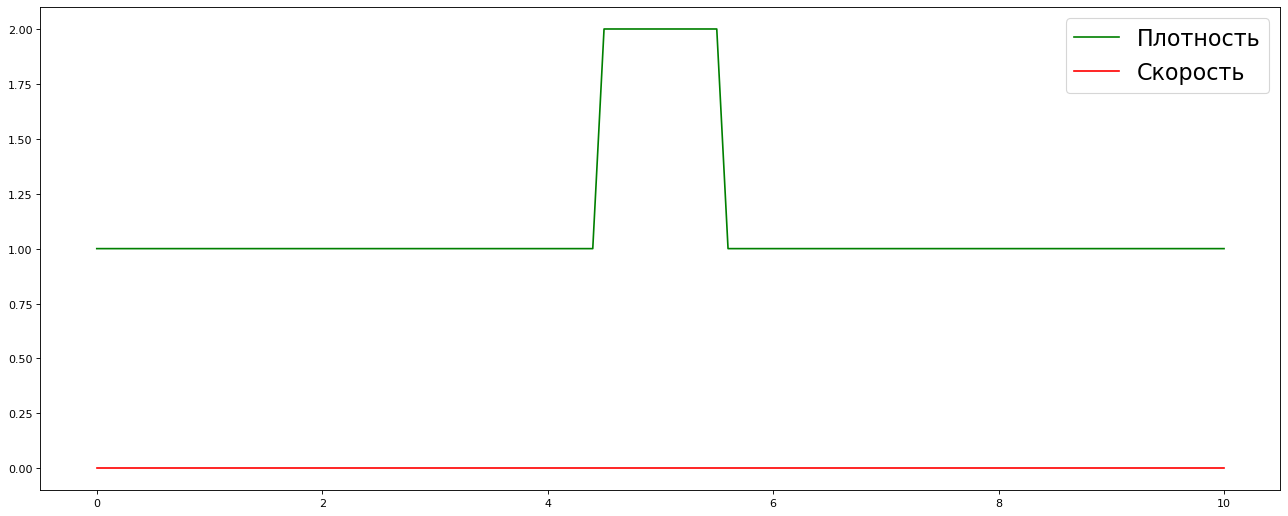
\includegraphics[width=\textwidth]{N_0.png}
\\
\newpage
t = 3, \(\Delta m\) = -4.712624e-01
\\
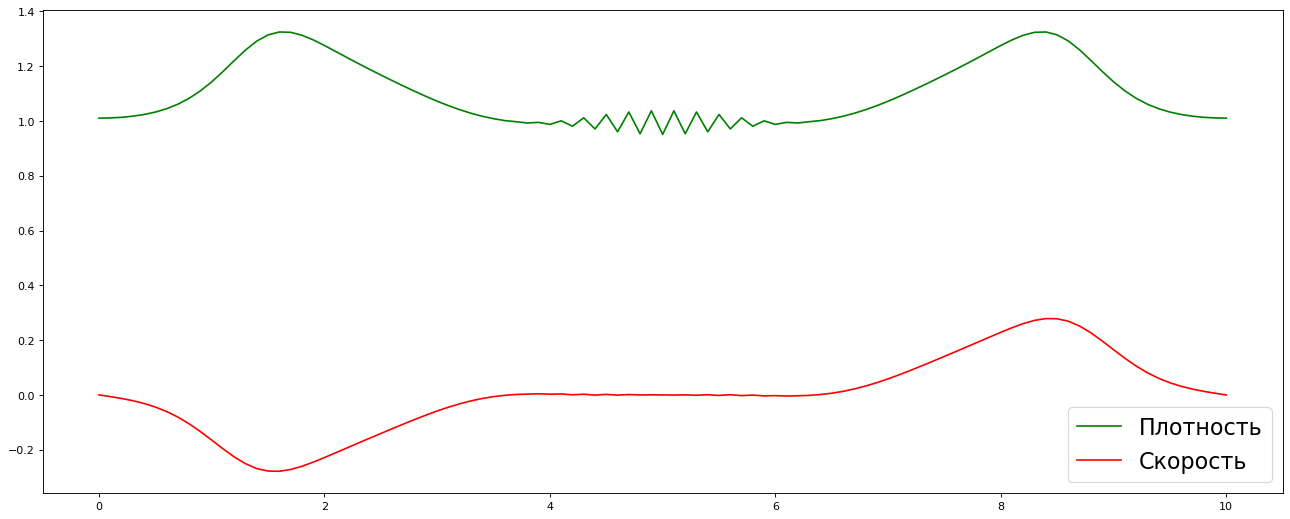
\includegraphics[width=\textwidth]{t_3.png}
\\

t = 10, \(\Delta m\) = -5.062991e-01
\\
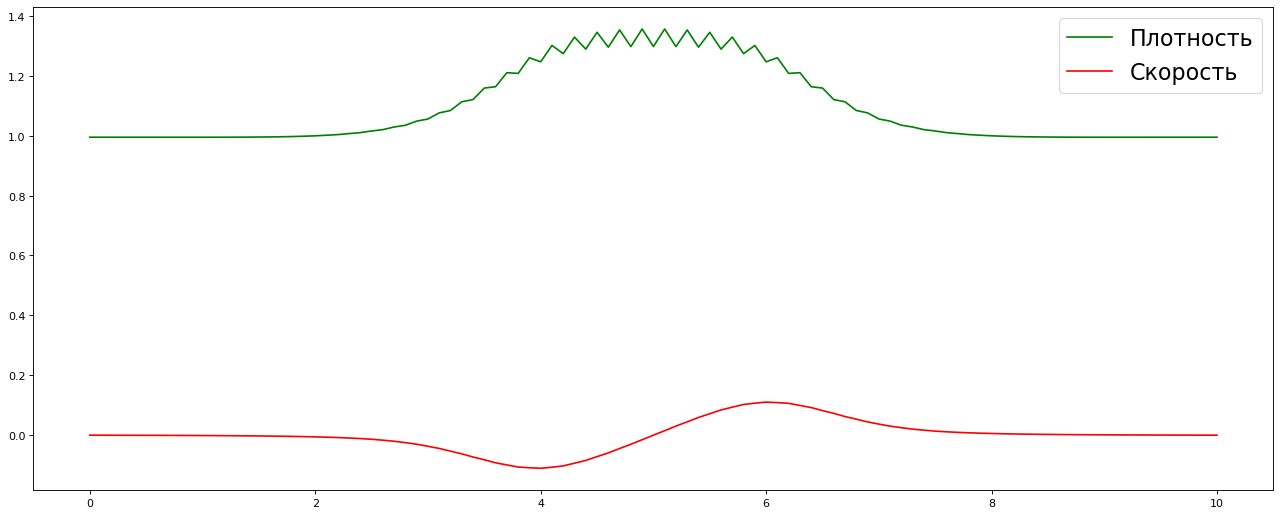
\includegraphics[width=\textwidth]{t_10.png}
\\

t = 50, \(\Delta m\) = -6.066234e-01
\\
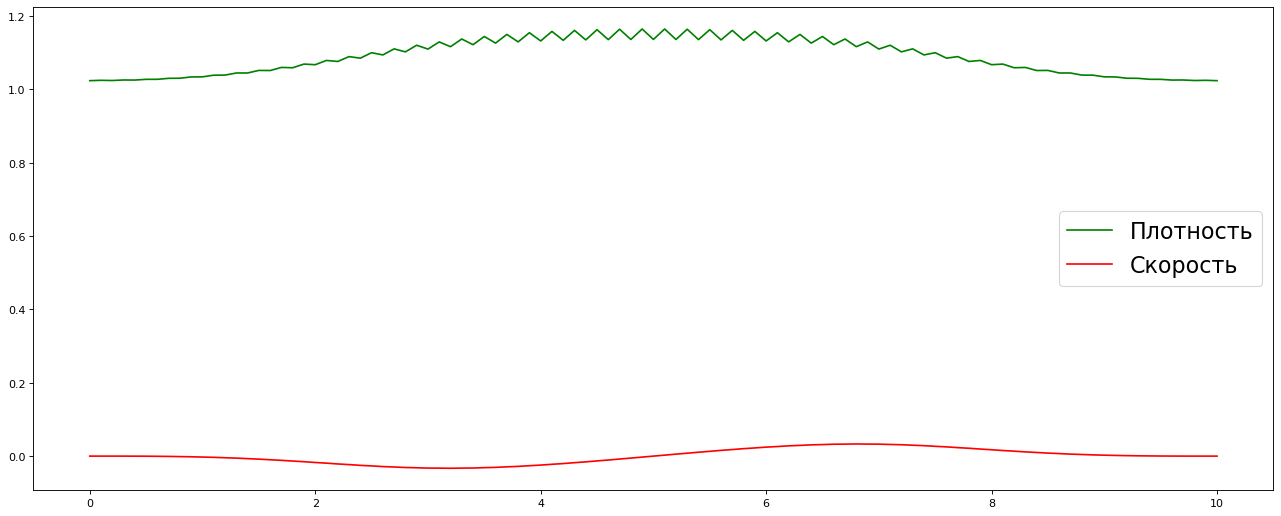
\includegraphics[width=\textwidth]{t_50.png}
\\
t = 100, \(\Delta m\) = -6.177132e-01
\\
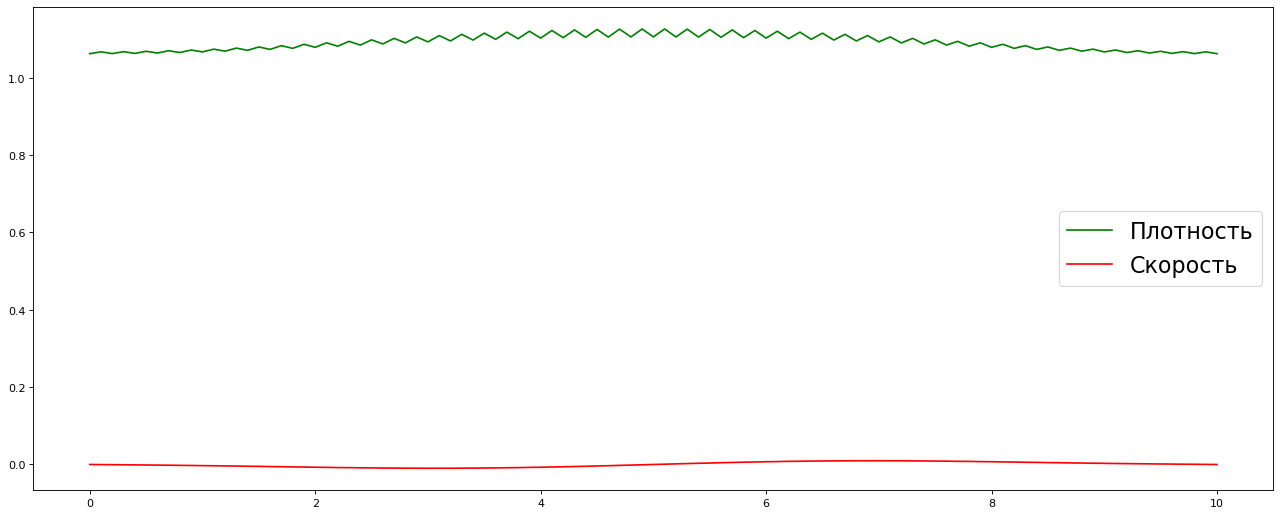
\includegraphics[width=\textwidth]{t_100.png}
\\
t = 500, \(\Delta m\) = -6.187471e-01
\\
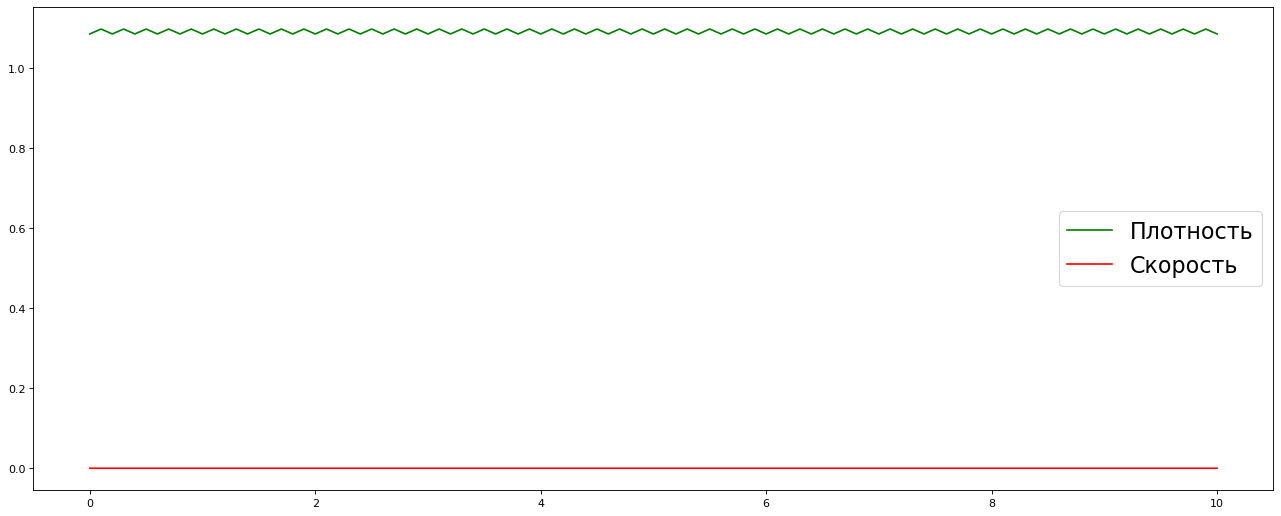
\includegraphics[width=\textwidth]{t_500.png}
\\
t = 1000, \(\Delta m\) = -6.187560e-01
\\
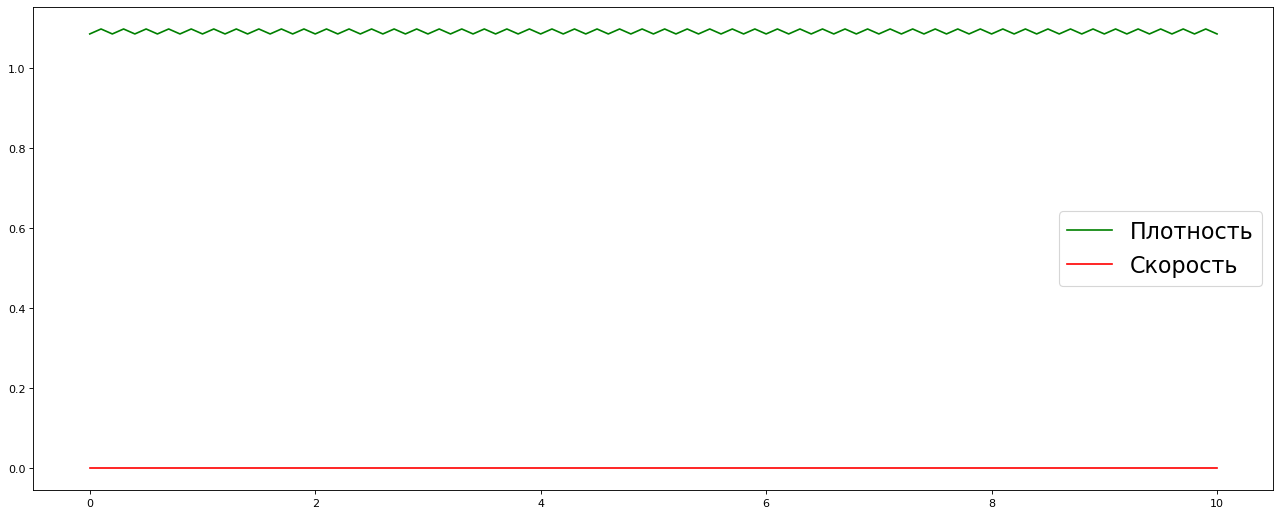
\includegraphics[width=\textwidth]{t_1000.png}
\\

\subsection{Задача с разрывной cкоростью}
\begin{equation*}
\begin{cases}
  \begin{gathered} 
   u_{0}(x)= \left[ 
      \begin{gathered} 
        0,\text{ } x<4.5 \text{ или } x>5.5 \hfill 
        \\ 
        1,\text{ } x \in [4.5,5.5] \hfill 
        \\ 
      \end{gathered} 
     \right. 
  \\

    \rho_{0}(x) \equiv 1, \text{ }  x \in  [0,10]  \hfill 
    \\
     u(t,0)=u(t,10)=0, \text{ } t \in [0,1] \hfill 
     \\ 
  \end{gathered} 
\end{cases}
\end{equation*}

Возьмём \(C = 1\) и \(\mu = 0.1\) шаг по \(x\) будет равен 0.1, шаг по \(t\) возьмём также 0.1. И будем смотреть стабилизацию решения. Под сходимостью будем подразумевать, что разница между максимальным и минимальным значением функций плотности и скорости меньше заданного \(\epsilon = 0.02\). Момент стабилизации 270.
\\
\\
\\
\\
\\
t = 0, \(\Delta m\) = 0
\\
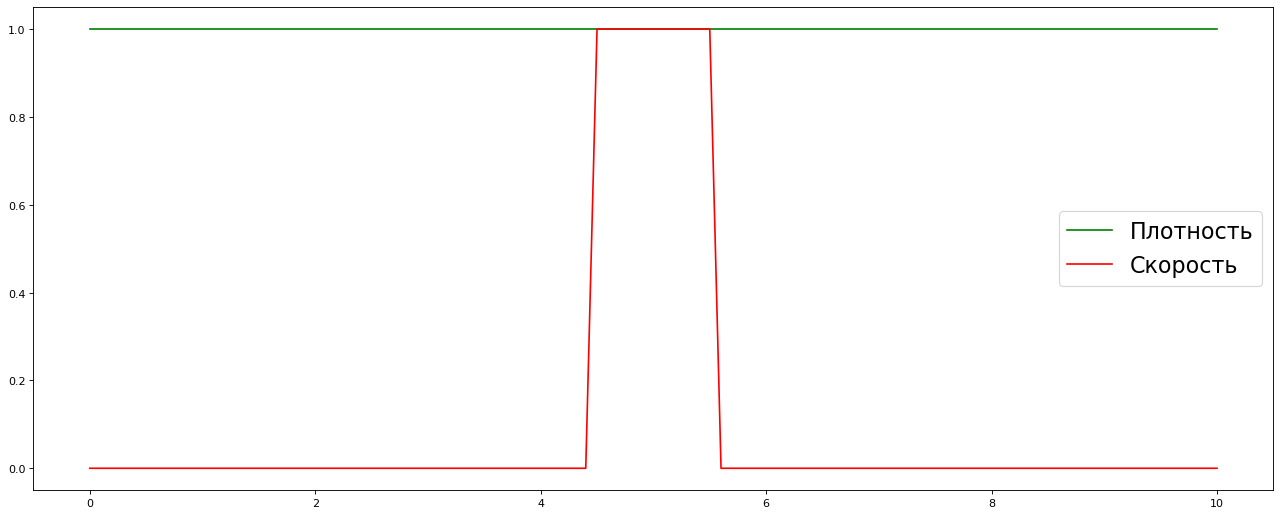
\includegraphics[width=\textwidth]{Ut_0.png}
\\
\newpage
t = 1, \(\Delta m\) = 4.397324e-02
\\
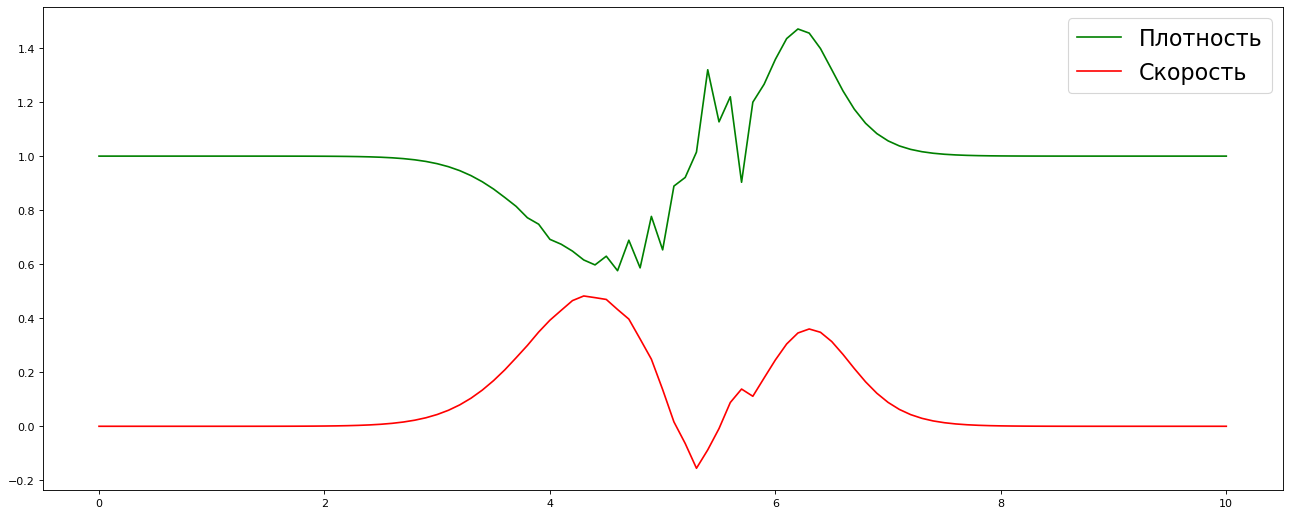
\includegraphics[width=\textwidth]{Ut_1.png}
\\

t = 5, \(\Delta m\) = -6.363942e-02
\\
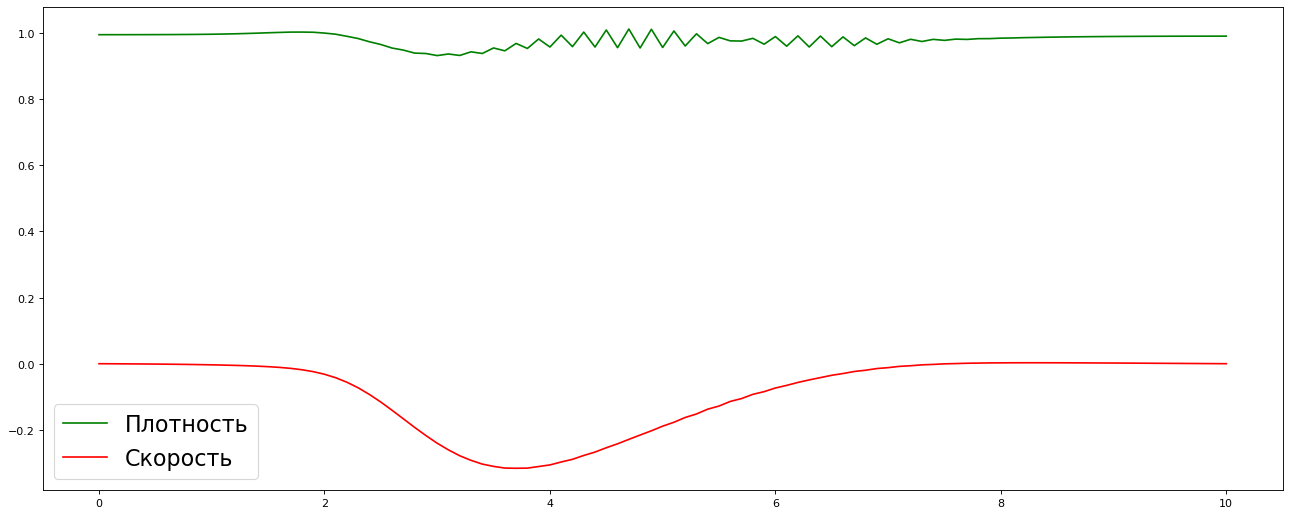
\includegraphics[width=\textwidth]{Ut_10.png}
\\

t = 50, \(\Delta m\) = --2.257169e-01
\\
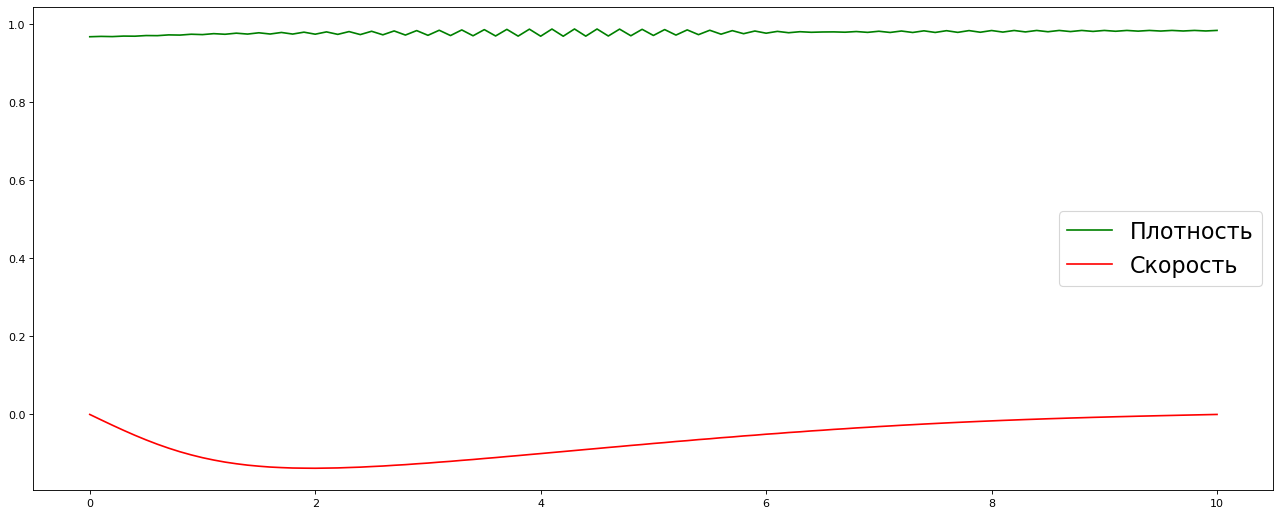
\includegraphics[width=\textwidth]{Ut_50.png}
\\
t = 100, \(\Delta m\) = -2.367071e-01
\\
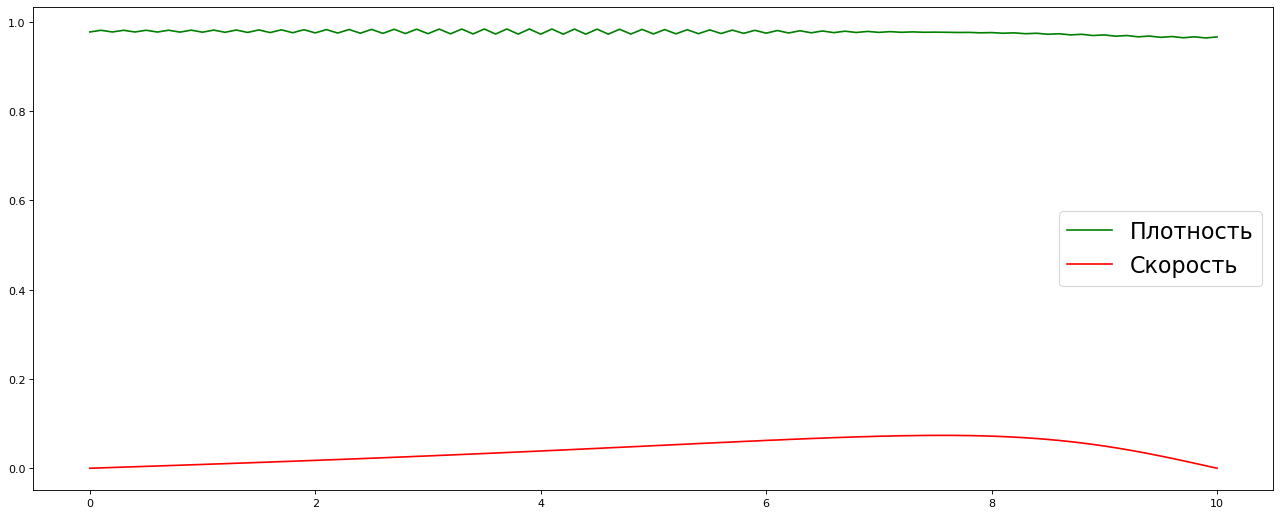
\includegraphics[width=\textwidth]{Ut_100.png}
\\
t = 500, \(\Delta m\) = -2.422271e-01
\\
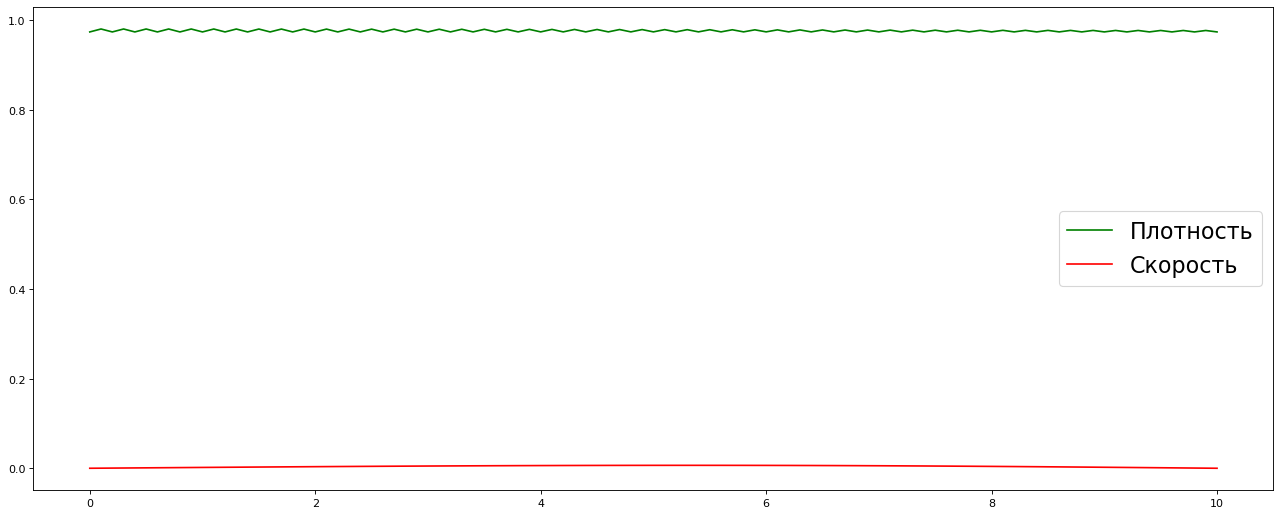
\includegraphics[width=\textwidth]{Ut_500.png}
\\
t = 1000, \(\Delta m\) = -2.422836e-01
\\
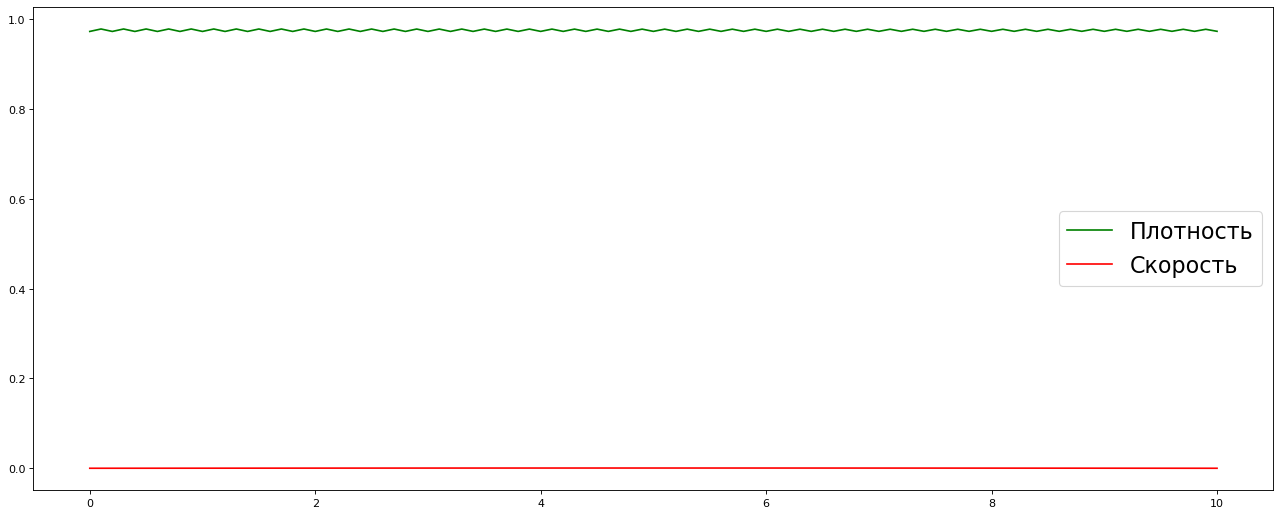
\includegraphics[width=\textwidth]{Ut_1000.png}
\\

\end{document}

